\documentclass[oneside,openany]{amsdtx}
\usepackage[margin=.75in]{geometry}
\usepackage{graphicx,float,amsmath,amssymb,url,multicol,booktabs,bm,array,enumitem}
\usepackage[dvipsnames]{xcolor}
\usepackage[allcolors=black]{hyperref}
\usepackage[T1]{fontenc}
\usepackage[utf8]{inputenc}
\usepackage[french,english]{babel}
\usepackage{lmodern}
\usepackage{siunitx}
\usepackage{listingsutf8}
\definecolor{b}{HTML}{3C78D8}\definecolor{B}{HTML}{08357E}\definecolor{g}{HTML}{38761D}
\definecolor{r}{HTML}{7A0101}\definecolor{phenolic}{HTML}{A65A2E}\definecolor{aluminium}{HTML}{A8B0B8}
\newcolumntype{L}[1]{>{\raggedright\arraybackslash}p{#1}}
\protected\def\code#1{\texttt{\detokenize{#1}}}
\sisetup{locale=FR,per-mode=symbol,range-phrase=--,range-units=single}
\setcounter{secnumdepth}{3}\setcounter{tocdepth}{2}
\title{~\\[-2em]\sc Préparation de la Simulation Thermochimique v0\\
du Nouveau Liner Phénolique}
\author{\sc MIT Rocket Team --- M. Nichitiu --- Simulations/Propulsion Solide}
\date{\sc 20 septembre 2026}

\begin{document}
\selectlanguage{french}
\maketitle
\begin{multicols}{2}
{\color{white}.}~~~~~~~~~~~~~~~~~
\includegraphics[scale=0.1]{logos/rtlogo.pdf}\\[1em]
~\vspace{3.3em}~\\[-4.6em]{\color{white}.}~~~~~
\includegraphics[scale=0.2]{logos/ansys.png}
\end{multicols}
~\\[-1em]
\tableofcontents
\vfill
\begin{center}\begin{minipage}{0.96\textwidth}\small
\textbf{Objet du document.} Ce rapport enregistre la préparation reproductible
de la première version du modèle du nouveau moteur. Il distingue strictement la
géométrie demandée des hypothèses reprises des simulations antérieures. Le
modèle natif Windows, le maillage, la chaîne de reprise et le précontrôle MAPDL
sont prêts, mais aucun calcul transitoire n'a été lancé. L'objectif principal
est de calculer, sans ambiguïté de vocabulaire, l'épaisseur de phénolique
retirée, l'épaisseur restante, la masse gazeuse issue de la pyrolyse et la masse
de carbone consommée à chaque instant.
\end{minipage}\end{center}
\vfill

\section{Définition du nouveau moteur}
\subsection{Dimensions imposées}
Le cahier des charges fourni pour cette étude contient trois diamètres :
\(D_{\mathrm{Al,ext}}=\SI{6.000}{in}\),
\(D_{\mathrm{Al,int}}=D_{\mathrm{ph,ext}}=\SI{5.625}{in}\) et
\(D_{\mathrm{ph,int}}=\SI{5.250}{in}\). Contrairement aux deux premières
simulations historiques, ces cotes sont bien traitées comme des \emph{diamètres}
et sont divisées par deux avant de devenir des coordonnées radiales.

\begin{table}[H]\centering
\caption{Interfaces radiales nominales.}
\begin{tabular}{L{5.0cm}rrr}\toprule
Interface & Diamètre [in] & Diamètre [mm] & Rayon [mm]\\\midrule
Alésage phénolique & 5,250 & 133,350 & 66,6750\\
Phénolique/aluminium & 5,625 & 142,875 & 71,4375\\
Extérieur aluminium & 6,000 & 152,400 & 76,2000\\\bottomrule
\end{tabular}
\end{table}

Il en résulte une unique couche phénolique de \SI{4.7625}{mm} et une enveloppe
d'aluminium de même épaisseur. Il n'y a ni époxy, ni deuxième phénolique, ni
contact artificiel intermédiaire. La simulation emploie un coupon axial de
\SI{50}{mm} et un secteur de \(0{,}10^\circ\), soit un facteur d'échelle de
3,600 vers l'anneau complet de même longueur. La longueur réelle du moteur
n'ayant pas été fournie, aucune masse totale de moteur n'est extrapolée au-delà
de ce segment de \SI{50}{mm}.

\begin{figure}[H]\centering
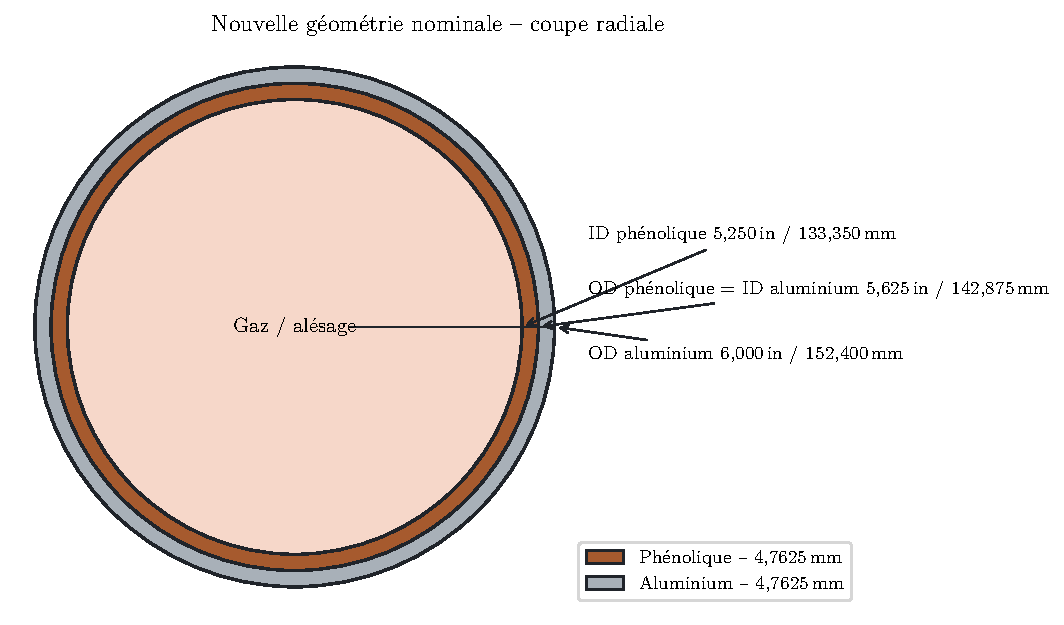
\includegraphics[width=.94\textwidth]{../analysis/newmotor_geometry_fr.pdf}
\caption{Coupe nominale des deux couches.}
\end{figure}

À titre de contrôle analytique, le segment complet de \SI{50}{mm} contient
\(V_{\mathrm{ph},0}=\SI{1.033208e-4}{m^3}\), soit
\(m_{\mathrm{ph},0}=\SI{0.129151}{kg}\) avec la densité de référence
\(\rho_v=\SI{1250}{kg.m^{-3}}\). Dans le secteur, la masse correspondante est
\SI{35.8753}{mg}. Ces valeurs sont des références de bilan, non des mesures de
la pièce fabriquée.

\subsection{Fichiers géométriques}
La base \code{geometry/newmotor_phenolic_v0.db} est une base native MAPDL 2026
R1 contenant les deux volumes collés. Elle a été créée sous Windows sans
maillage et sans commande \code{SOLVE}. Son générateur autonome,
\code{model/generate_geometry_mapdl.inp}, reste la source géométrique lisible.
La base d'échange utilise l'axe global Z; le maillage analytique du solveur
utilise l'axe global Y. Une rotation rigide relie les deux et ne change aucune
dimension ni condition thermique.

\section{Domaine de calcul et maillage}
\subsection{Choix de discrétisation}
Le maillage est structuré, conforme à l'interface et constitué exclusivement
d'hexaèdres thermiques linéaires SOLID70. Les deux matériaux partagent les
nœuds de l'interface : aucun élément de contact n'est nécessaire. Le
phénolique comporte 240 rangées radiales, soit
\[
\Delta r_{\mathrm{ph}}=\frac{\SI{4.7625}{mm}}{240}
=\SI{19.84375}{\micro m}.
\]
L'aluminium comporte 64 rangées de \SI{74.4141}{\micro m}. L'axe est découpé
en 250 intervalles de \SI{0.20}{mm} et l'angle en deux intervalles. Chaque
rangée phénolique exposable possède ainsi 500 faces.

\begin{figure}[H]\centering
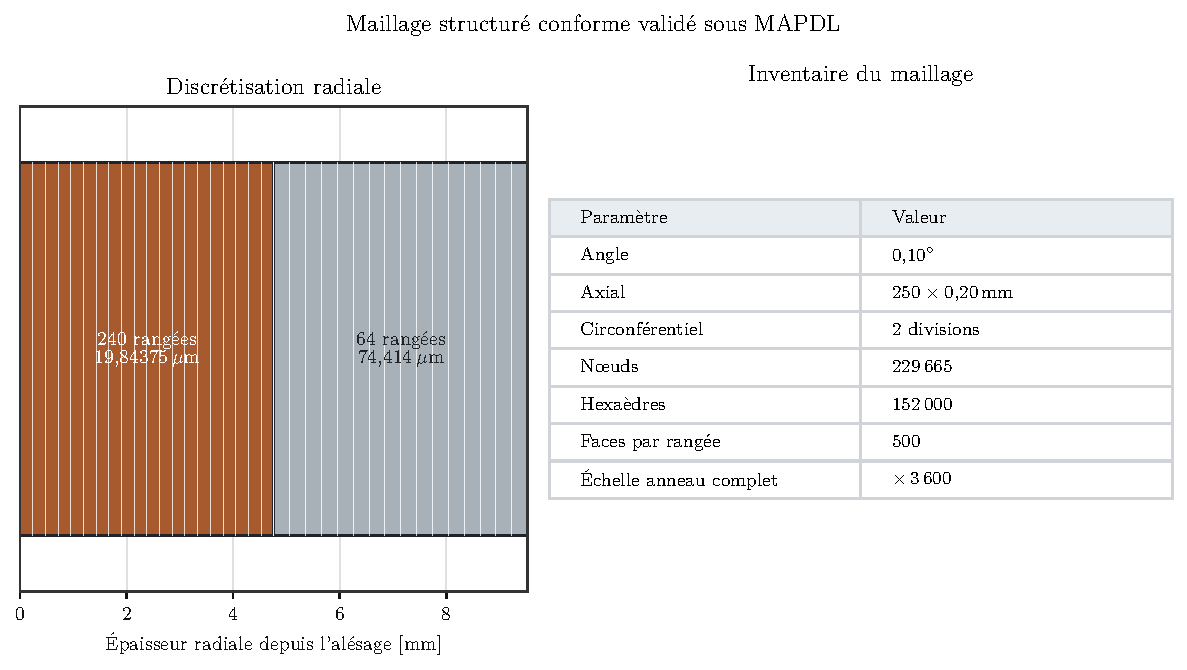
\includegraphics[width=.98\textwidth]{../analysis/newmotor_mesh_fr.pdf}
\caption{Résolution radiale et inventaire du maillage final.}
\end{figure}

Le modèle final comporte 229,665 nœuds et 152,000 hexaèdres, dont 120,000
dans le phénolique et 32,000 dans l'aluminium. Le premier essai à 100
divisions axiales produisait un rapport d'aspect de 25,2 et a été archivé dans
le répertoire temporaire. Le passage à 250 divisions ramène ce rapport près de
10. Le précontrôle MAPDL natif du modèle final s'achève avec zéro avertissement
et zéro erreur.

\subsection{Pourquoi un secteur de 0,10 degré}
Deux divisions angulaires suffisent pour conserver une topologie 3D et des
faces de convection explicites, tandis que les 240 rangées radiales donnent la
résolution nécessaire à la suppression progressive. Ce secteur ne peut pas
représenter une non-uniformité circonférentielle à grande échelle. Il convient
donc pour une réponse axisymétrique locale; toute fissure, joint ou jet local
impose un domaine angulaire plus large.

\section{Modèle thermochimique prévu}
\subsection{Pyrolyse du phénolique}
La loi UserMatTh conserve les états internes de conversion et fournit, pour
chaque élément vivant, la conversion \(\alpha\), la production gazeuse et les
termes énergétiques. Les densités de référence vierge et carbonisée valent
respectivement \SI{1250}{kg.m^{-3}} et \SI{600}{kg.m^{-3}}; l'enthalpie de
pyrolyse provisoire vaut \SI{418}{kJ.kg^{-1}}. Les propriétés thermiques
dépendent de la température et de la conversion.

La face chaude reçoit par défaut \(T_g=\SI{2230.85}{\degreeCelsius}\) et
\(h_0=\SI{1000}{W.m^{-2}.K^{-1}}\). Le soufflage réduit le coefficient par une
fonction continue du flux gazeux. La face externe échange avec l'ambiance à
\SI{22}{\degreeCelsius} par convection
(\(h=\SI{8}{W.m^{-2}.K^{-1}}\)) et rayonnement
(\(\varepsilon=0{,}25\)).

\begin{center}\fbox{\begin{minipage}{0.92\textwidth}\small
\textbf{Limite de qualification.} La pression de chambre, la composition des
gaz et la cinétique d'oxydation du carbone ne sont pas encore disponibles. La
loi de consommation du charbon est donc explicitement marquée
\code{EXPLORATORY_NOT_CALIBRATED}. Les résultats peuvent comparer des variantes
et vérifier les bilans, mais ne deviennent prédictifs qu'après calibration sur
le matériau et le moteur réels.
\end{minipage}}\end{center}

\subsection{Suppression d'une rangée}
Une rangée n'est désactivée que lorsque sa masse solide résiduelle, après
pyrolyse et consommation du carbone, tombe sous 0,1\,\% de sa masse vierge
initiale. La suppression a lieu après acceptation du pas convergé et est
réappliquée après restauration du checkpoint. Cette règle remplace la décision
fragile fondée uniquement sur une moyenne de conversion.

Le pas de couplage nominal est \SI{0.05}{s}; le solveur peut descendre à
\SI{0.0005}{s}. L'horizon de référence est \SI{7}{s}, repris uniquement pour
permettre la comparaison avec l'étude précédente. Il devra être remplacé dans
une nouvelle version, avant tout lancement, si la durée de combustion réelle
du nouveau moteur diffère.

\section{Grandeurs principales et bilans}
\subsection{Épaisseur restante}
Après \(N_k(t)\) rangées acceptées pour suppression,
\[
s_{\mathrm{ret}}(t)=N_k(t)\,\Delta r_{\mathrm{ph}},\qquad
s_{\mathrm{rest}}(t)=s_0-s_{\mathrm{ret}}(t),
\quad s_0=\SI{4.7625}{mm}.
\]
La résolution de l'épaisseur discrète est donc \SI{19.84375}{\micro m}. La
coordonnée de la paroi chaude vaut \(R_h(t)=R_i+s_{\mathrm{ret}}(t)\).

\subsection{Masse de phénolique consommée}
Trois quantités ne doivent pas être confondues :
\begin{enumerate}[nosep]
\item la masse gazeuse cumulée issue de la pyrolyse;
\item la masse de carbone consommée sur la surface exposée;
\item la masse vierge équivalente des rangées géométriquement retirées.
\end{enumerate}
Pour un anneau complet de longueur \(L\), cette dernière vaut
\[
m_{\mathrm{ret},0}(t)=\rho_v\,\pi L
\left[\bigl(R_i+s_{\mathrm{ret}}(t)\bigr)^2-R_i^2\right].
\]
Le journal conserve les valeurs du secteur et les valeurs multipliées par
3,600. Le bilan ferme à chaque pas entre masse initiale, solide restant, gaz
de pyrolyse, carbone consommé et résidu éjecté. Une erreur supérieure à la
tolérance bloque automatiquement la suite du calcul.

\subsection{Sorties prévues}
Le fichier \code{newmotor_v0_history.csv} sera réécrit atomiquement après chaque
pas accepté. Il contient notamment le temps, le numéro de rangée, l'épaisseur
retirée et restante, les masses sectorielles et anneau complet, la température
de surface, \(\alpha_{\mathrm{moy}}\), \(\alpha_{\min}\), le coefficient de
film, les puissances, les résidus de bilans et les éventuels avertissements.
Un fichier JSON immuable est conservé pour chaque checkpoint; le CSV n'est
qu'une vue reconstruite de ces enregistrements.

Les figures de résultats seront générées à partir de ces états convergés :
épaisseur restante et retirée en fonction du temps, composantes de masse
consommée, vitesse de récession, température et soufflage, profils radiaux de
température/conversion, ainsi que distance entre la surface et les fronts de
pyrolyse 90, 95 et 99\,\%. La naissance du front de récession sera marquée par
une ligne verticale.

\section{Exécution Windows, pause et reprise}
Tous les gros fichiers sont isolés dans \code{v0/ansystmp}, ignoré par Git. Le
dossier \code{v0} est mappé sous Windows sur le lecteur \code{V:}; le runtime
est \code{V:\textbackslash ansystmp\textbackslash windows}. Il ne contient
aucune référence vers l'ancien projet. Les sources UserMatTh et la DLL sont
copiées localement.

Avant le premier calcul, \code{launch_v0.ps1 -Preflight} vérifie les empreintes
des entrées, le maillage, la licence locale \code{1055@localhost} et charge le
deck complet sans \code{SOLVE}. Le précontrôle du 20 septembre 2026 confirme
229,665 nœuds, 152,000 éléments, zéro avertissement et zéro erreur. Aucun
processus de calcul n'est actuellement actif et aucun \code{state.json} de
simulation n'a été créé.

Le lancement exige l'option explicite \code{-Run} et 10 rangs DMP. Le script
refuse de démarrer si ANSYS/MPI est déjà présent. Six générations de restart
sont conservées. \code{request_pause.ps1} demande un arrêt au prochain
macro-pas accepté; \code{-Run -Resume} n'est autorisé qu'à partir d'un état
\code{PAUSED_AT_CHECKPOINT} dont les entrées sont inchangées.

\section{État de préparation et prochaines décisions}
\begin{table}[H]\centering
\begin{tabular}{L{7.2cm}L{5.4cm}}\toprule
Élément & État\\\midrule
Géométrie à deux volumes & créée et archivée dans une base MAPDL native\\
Maillage structuré & validé : 229,665 nœuds, 152,000 hexaèdres\\
Précontrôle Windows & terminé, 0 avertissement, 0 erreur, aucun solve\\
Entrées de calcul & scellées par SHA-256\\
Pause/reprise & préparée au checkpoint accepté\\
Rapports FR/EN & compilés à partir des mêmes paramètres\\
Calcul transitoire & non lancé; autorisation explicite encore nécessaire\\\bottomrule
\end{tabular}
\end{table}

Avant de lancer, il reste souhaitable de fournir la durée de combustion réelle,
la pression de chambre, la composition gazeuse et les propriétés mesurées du
phénolique. Sans ces données, le calcul v0 est volontairement une référence
exploratoire de sept secondes. Sa structure est néanmoins prête à répondre à
la question principale : combien de phénolique a été transformé ou retiré, et
quelle épaisseur saine reste à chaque instant ?

\end{document}

